
\subsection{Integration With ZGC}
\label{sec:future-work:integration}

As highlighted thoroughly throughout the report, the natural next step from this work is to integrate it into ZGC. As highlighted in Section~\ref{sec:individual_contrubitons}, N. Gärds~\cite{niclas_report} has, in parallel to when this work was performed, investigated integrating an allocator into ZGC. His work focuses on the challenges and opportunities of integrating any allocator into ZGC, not specifically the optimized TLSF allocator described in this work. As such, it would be interesting to use the findings of Gärds' to integrate the optimized TLSF allocator into ZGC so that its impact may be fully understood.

\subsection{Smaller Minimum Allocation Size}
\label{sec:future-work:lilliput}

The smallest possible unit of allocation inside ZGC is at the time or writing 16 bytes. This limit is due to the fact that object headers in Java are 16 bytes large, or 128 bits. However, work is currently in progress to reduce the size of the object header down to 64 bits or less through project Lilliput~\cite{lilliput}. Since Lilliput is still work in progress, the smaller allocation size of 8 bytes has not been supported in the general nor optimized version of the allocator.

Blocks that are smaller than 16 bytes require very little information on their particular size, which goes against using 8 bytes for storing size information, as detailed in Section~\ref{sec:adaptations_impl:0-byte-header}. Furthermore, as discussed in Section~\ref{sec:tlsf} regarding the design of TLSF and continuing in Section~\ref{sec:adaptations:architectural-considerations} on architectural adjustments, there is now an extra bit available for storing metadata inside block headers when aligning allocations to 8 bytes instead of 4 bytes. One might use this third metadata bit as a binary property to indicate whether a block is the smallest possible size, 8 bytes, or not. If the bit is set, the size field in the block header can be replaced with the next and prev pointers, making it possible to store all metadata about the block inside 8 bytes.

% TODO: Fix image
%\begin{figure}[H]
    %\centering
    %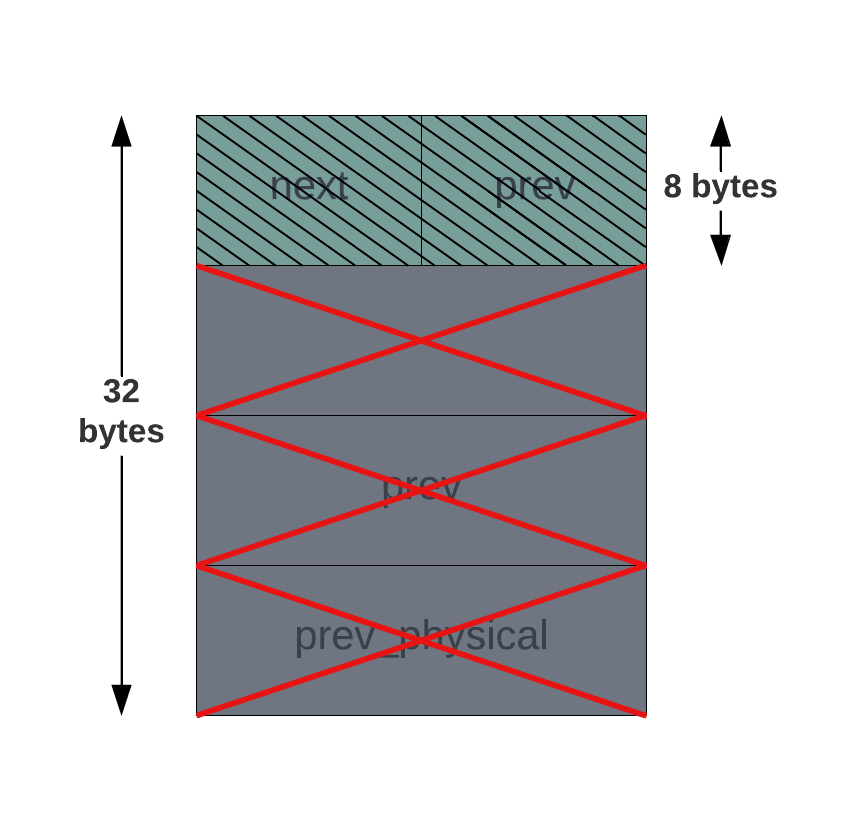
\includegraphics[width=0.5\textwidth]{figures/blockheader_lilliput.png}
    %\caption{Illustration of what the block header could contain after adjustments for Lilliput.}
    %\label{fig:lilliput_block_header}
%\end{figure}

\subsection{Addressing Starvation}
\label{sec:future-work:starvation}

One of the main selling points of TLSF is its bounded worst-case performance, which makes it an attractive choice in real-time systems where long response times are undesirable. The TLSF algorithm is able to achieve its bounded performance because it has no loops in its design. However, when introducing concurrency using a lock-free mechanism, as described in Section~\ref{sec:adaptations_impl:concurrency} this is no longer the case. The lock-free implementation of the free-lists in the optimized version requires adding a loop to make sure that the CAS instruction eventually succeeds. Thus, for concurrent use-cases, the worst-case performance of the optimized allocator is not bounded and may end up in cases where all but one thread starve. 

To solve the issue of starvation, a strategy worth exploring is combining the lock-free implementation with a wait-free one that guarantees progress for every thread, thereby preventing starvation. A. Kogan and E. Petrank~\cite{fast_wait_free} propose a way to do this by creating fast wait-free data structures, which can be applied to the lock-free solution that we have designed. The idea is to execute the efficient lock-free version most of the time, and execute a slower wait-free version only when things go wrong. This would make sure that per-thread progress is guaranteed and that threads do not end up starving.

%%% Local Variables:
%%% mode: latex
%%% TeX-master: "main"
%%% End:
